\documentclass[a4paper,10pt,twoside]{article}

\usepackage[english]{babel}
\usepackage{amssymb}
\usepackage{fancyhdr}
\usepackage{graphicx}
\usepackage[ocgcolorlinks]{hyperref}
\usepackage{todonotes}
\usepackage{caption}
\usepackage{subcaption}

\pagestyle{fancy}
\fancyhead{}
\fancyfoot{}
\fancyhead[RE,LO]{de Kok \& Methenitis}
\fancyhead[RO,LE]{Week 3}
\fancyfoot[RE]{\thepage$\quad \square$}
\fancyfoot[LO]{$\square \quad$\thepage}

\title{Report for Week 3 \\\normalsize $k$-means \& Bag-of-Visual words\\ or how to create a Google Goggles-like system}

\author{Patrick de Kok (5640318) \and Georgios Methenitis (10407537)}

\begin{document}
\maketitle
\thispagestyle{empty}

\section{Individual steps of $k$-means}
In the first step of the assignment we are focusing on implementing the $k$-means algorithm and check the results of these individual steps of the algorithm. Choosing the best parameter $k$ always depends on the application. In this example where we have to cluster the datapoints which consist of three clusters, it is best to use $k=3$ but this parameter varies for different applications. For example, image segmentation often needs around 10 (see for instance~\cite{Methenitis2013}) clusters to be computed. There is also a big trade off between number of clusters and the performance of the algorithm. We know that for a large value for $k$ algorithm takes long time to converge.
A really serious aspect of this algorithm is the relation between its random starting points in the state space and the solution that it gives. There is a big dependency and the algorithm can converge to a different final solutions depending on the starting points for the centers. Figure~\ref{fig:kmeanssimple} depicts the results of the three steps of the algorithm with different values for $k$.


\begin{figure}
  \begin{subfigure}{1.00\textwidth}
    \centering
    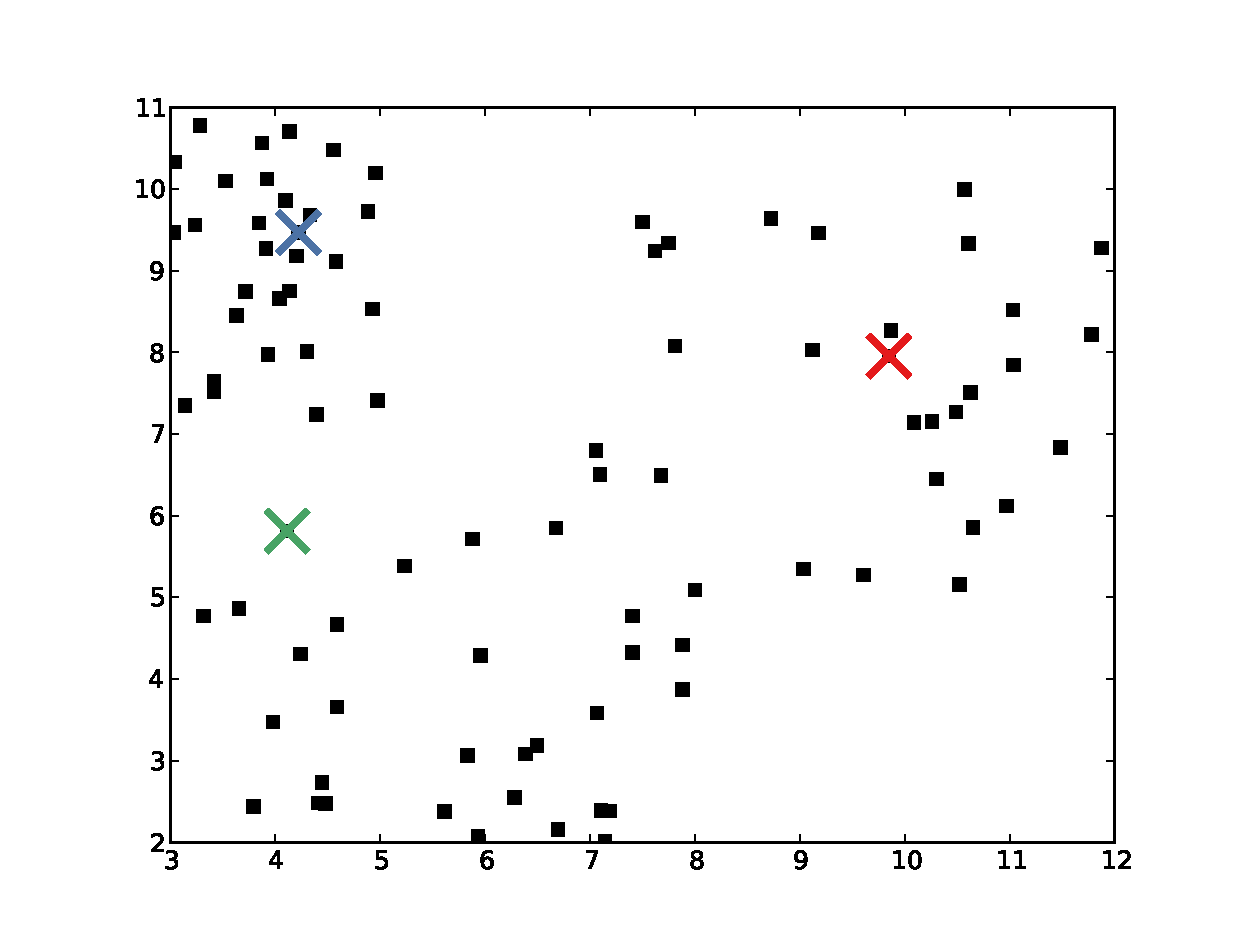
\includegraphics[width=.32\textwidth,height=.3\textheight,keepaspectratio]{figure_1.eps}	
    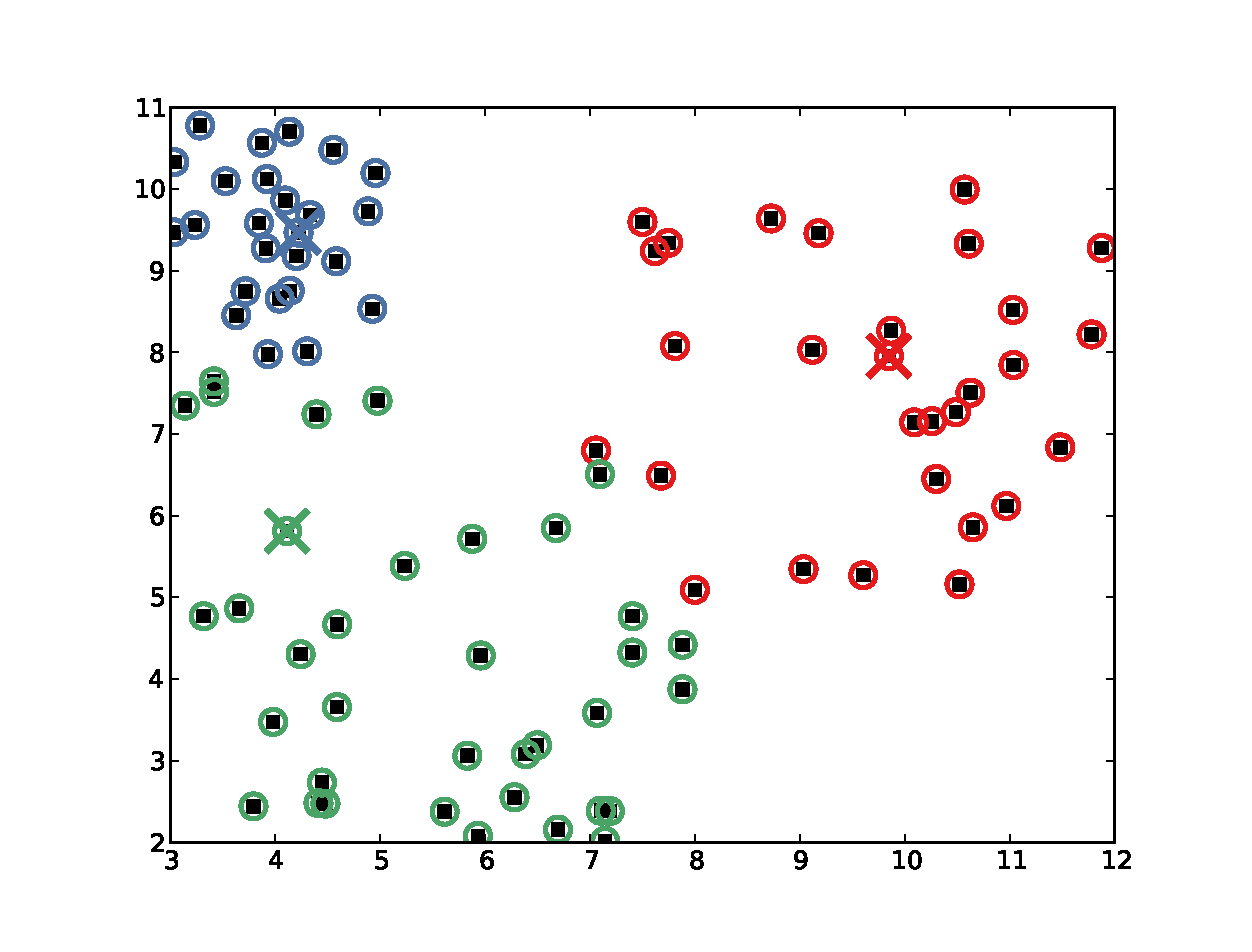
\includegraphics[width=.32\textwidth,height=.3\textheight,keepaspectratio]{figure_2.eps}
    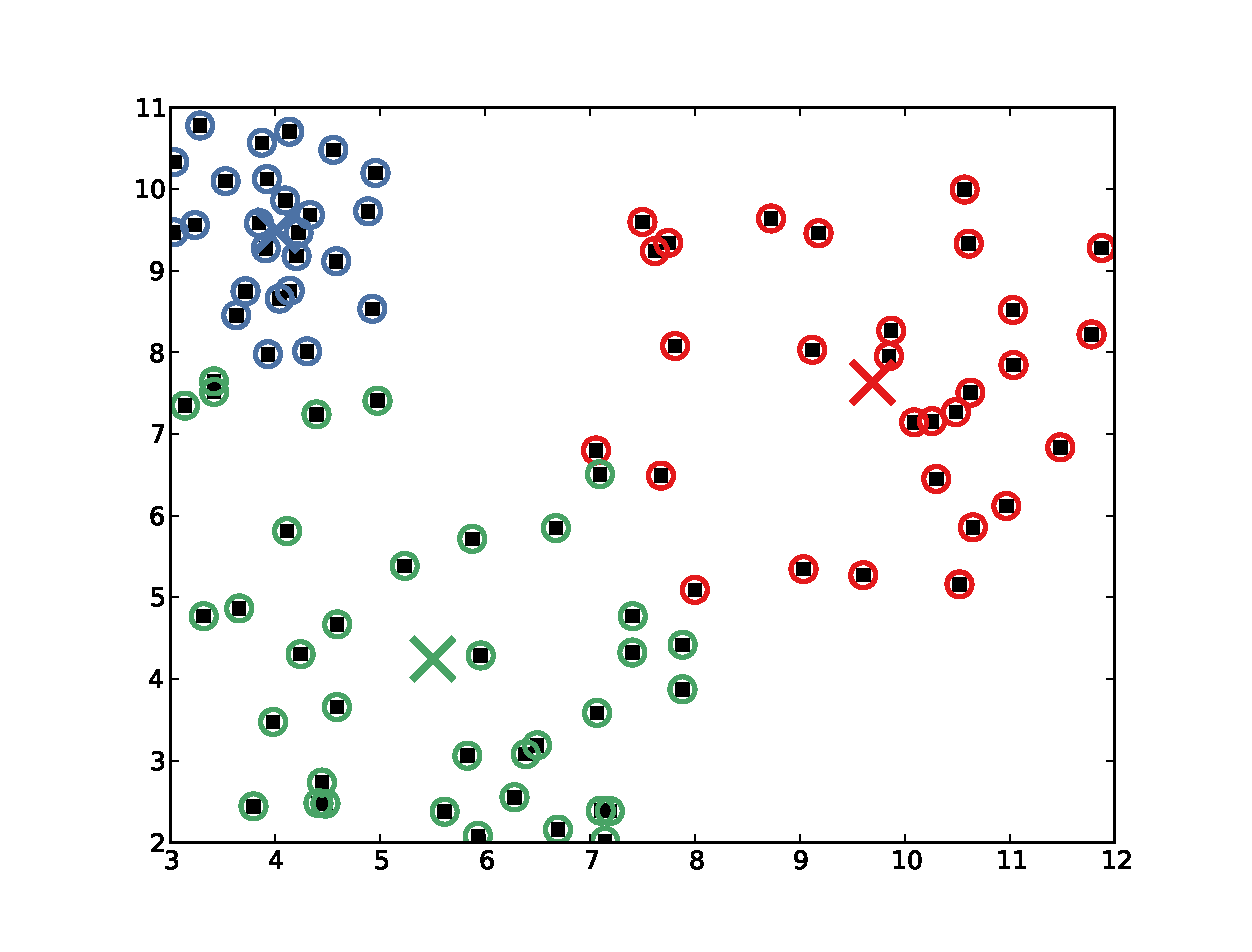
\includegraphics[width=.32\textwidth,height=.3\textheight,keepaspectratio]{figure_3.eps}
    \caption{K=3}
  \end{subfigure}
  \begin{subfigure}{1.00\textwidth}
    \centering
    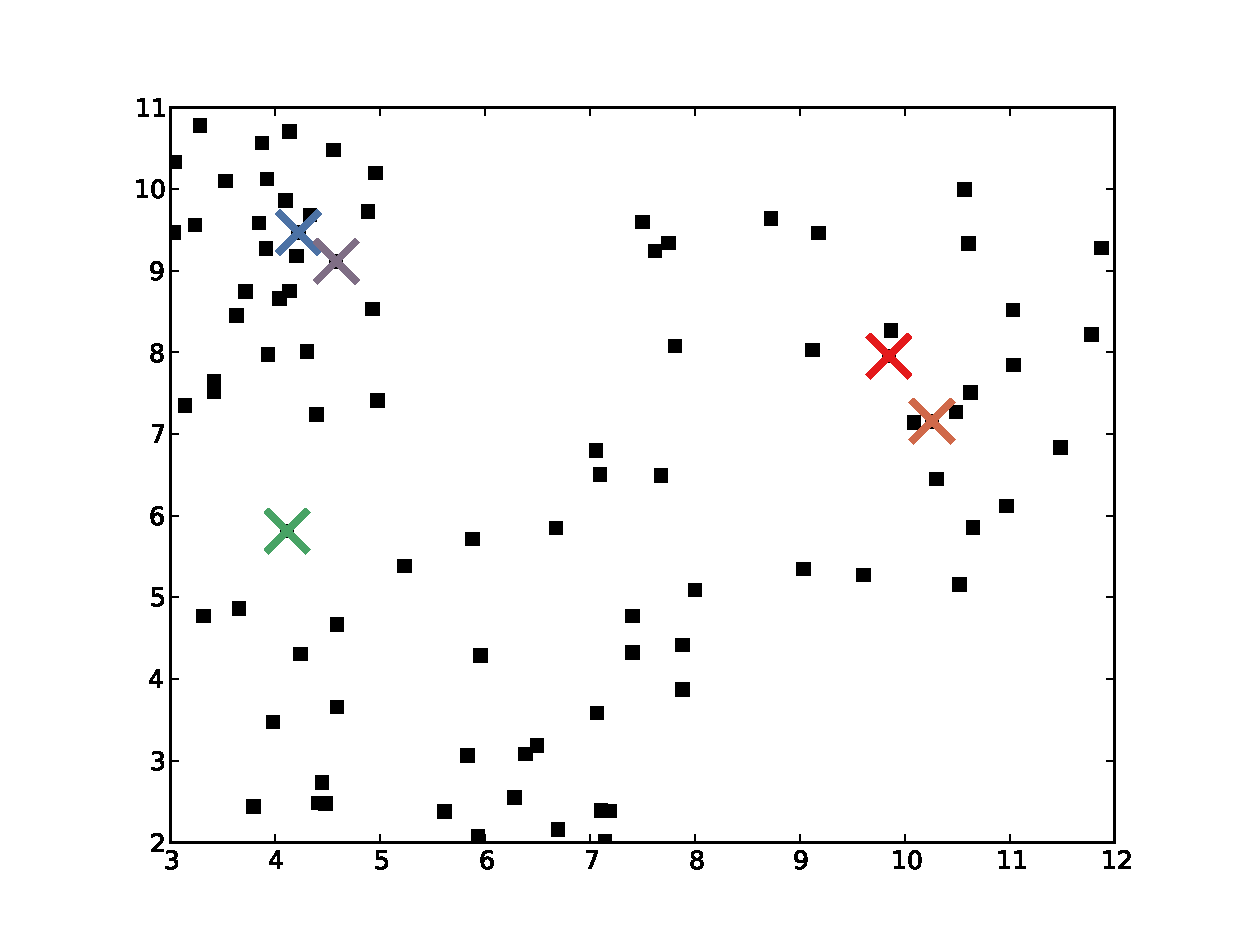
\includegraphics[width=.32\textwidth,height=.3\textheight,keepaspectratio]{figure_4.eps}
    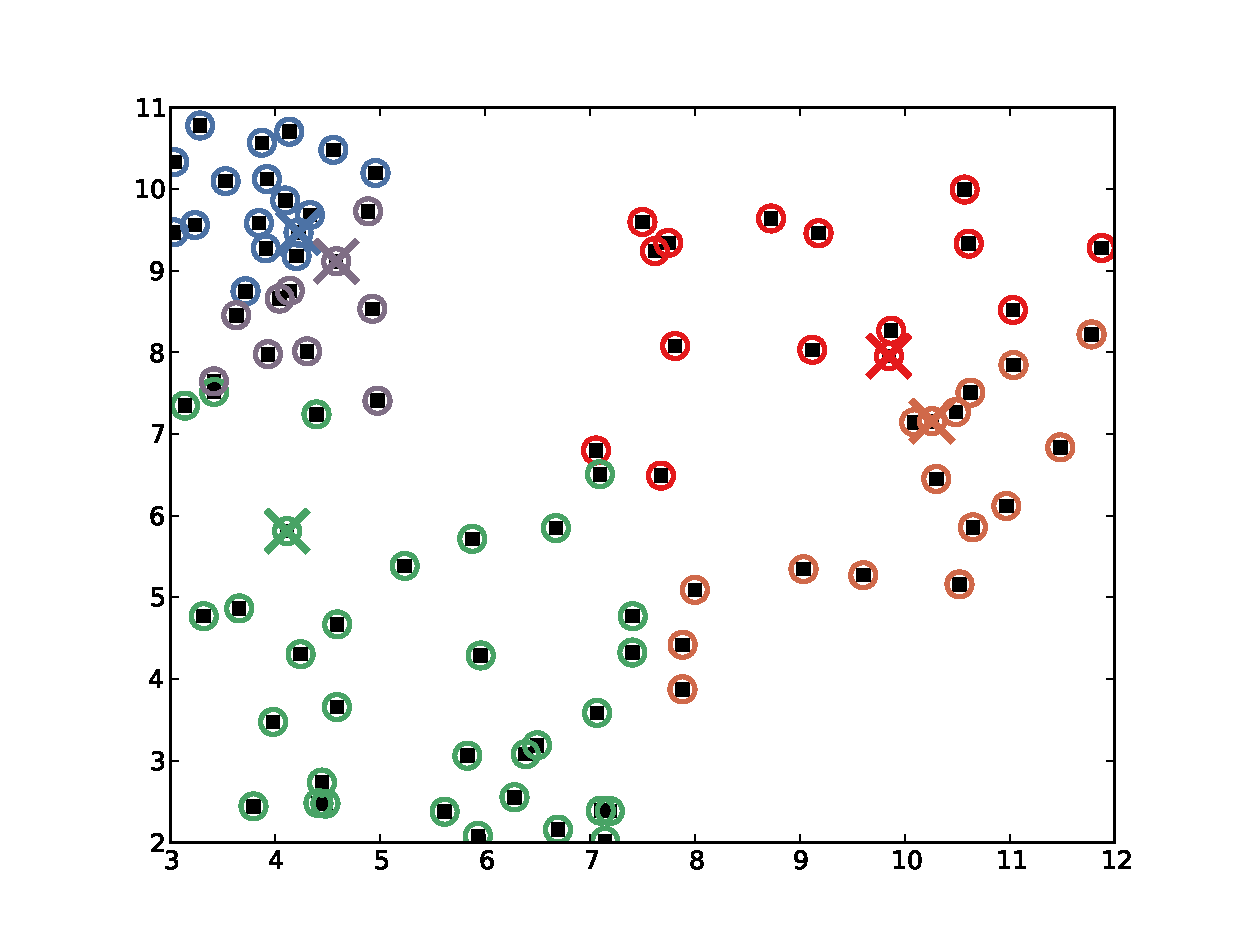
\includegraphics[width=.32\textwidth,height=.3\textheight,keepaspectratio]{figure_5.eps}
    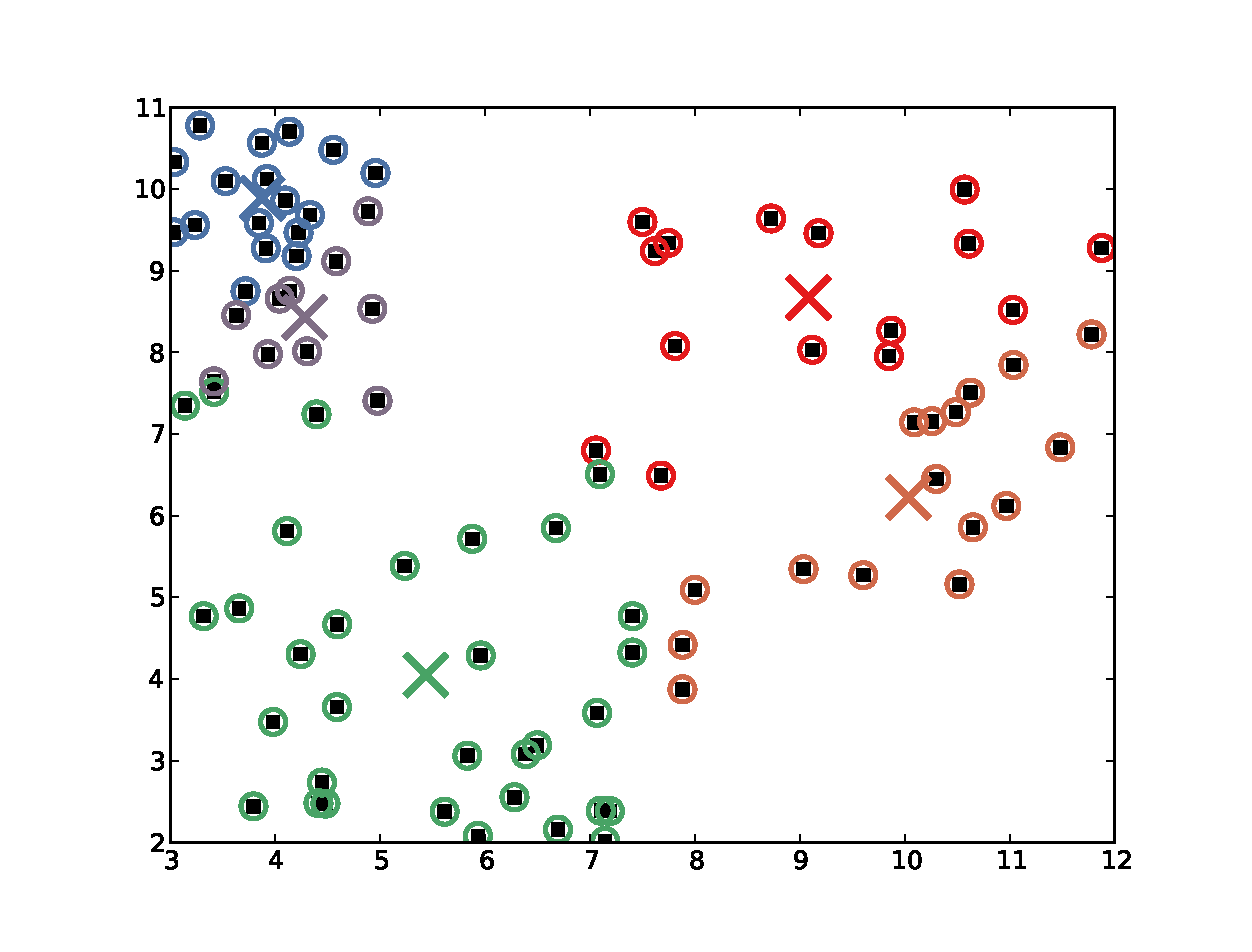
\includegraphics[width=.32\textwidth,height=.3\textheight,keepaspectratio]{figure_6.eps}
    \caption{K=5}
  \end{subfigure}
  \begin{subfigure}{1.00\textwidth}
    \centering
    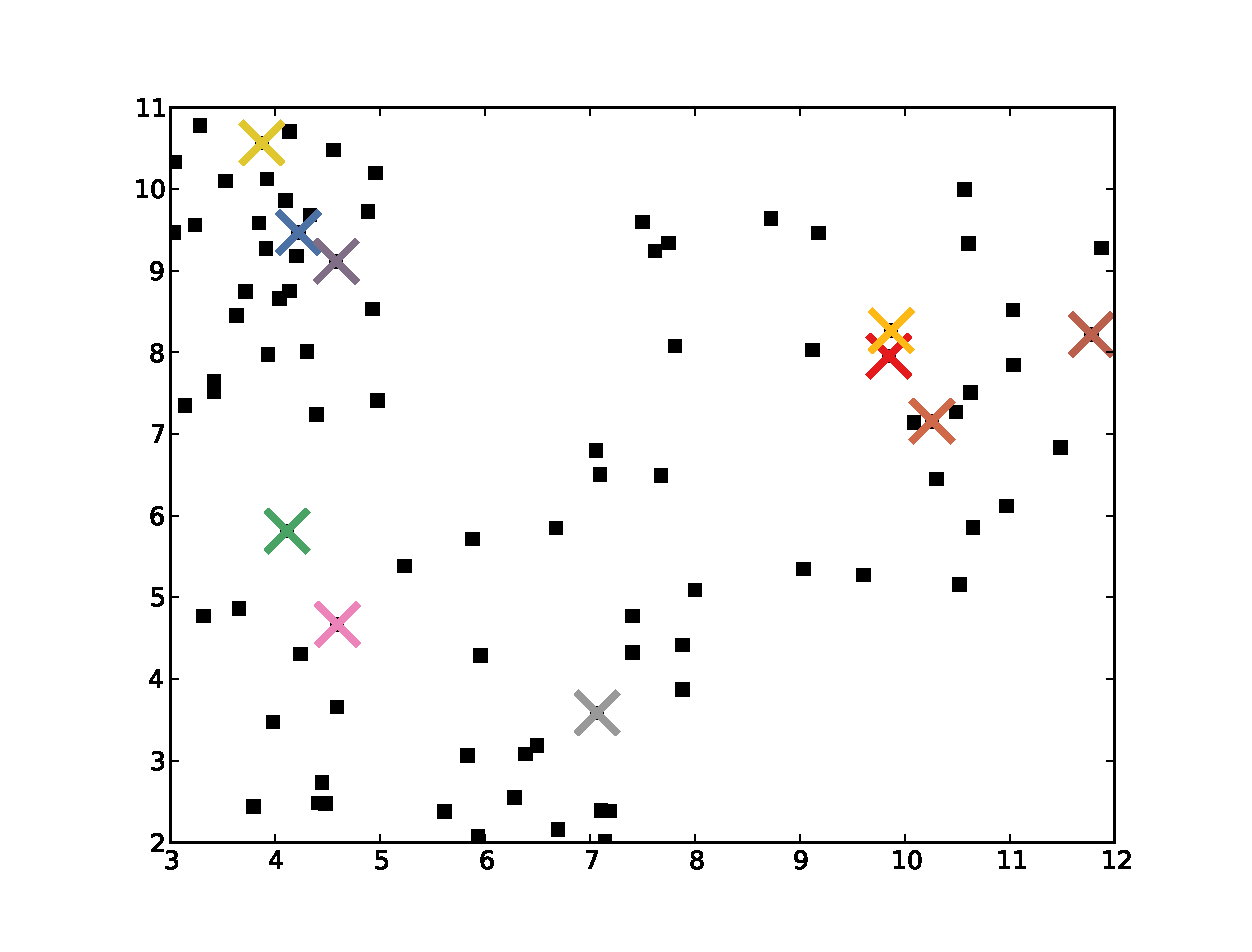
\includegraphics[width=.32\textwidth,height=.3\textheight,keepaspectratio]{figure_7.eps}
    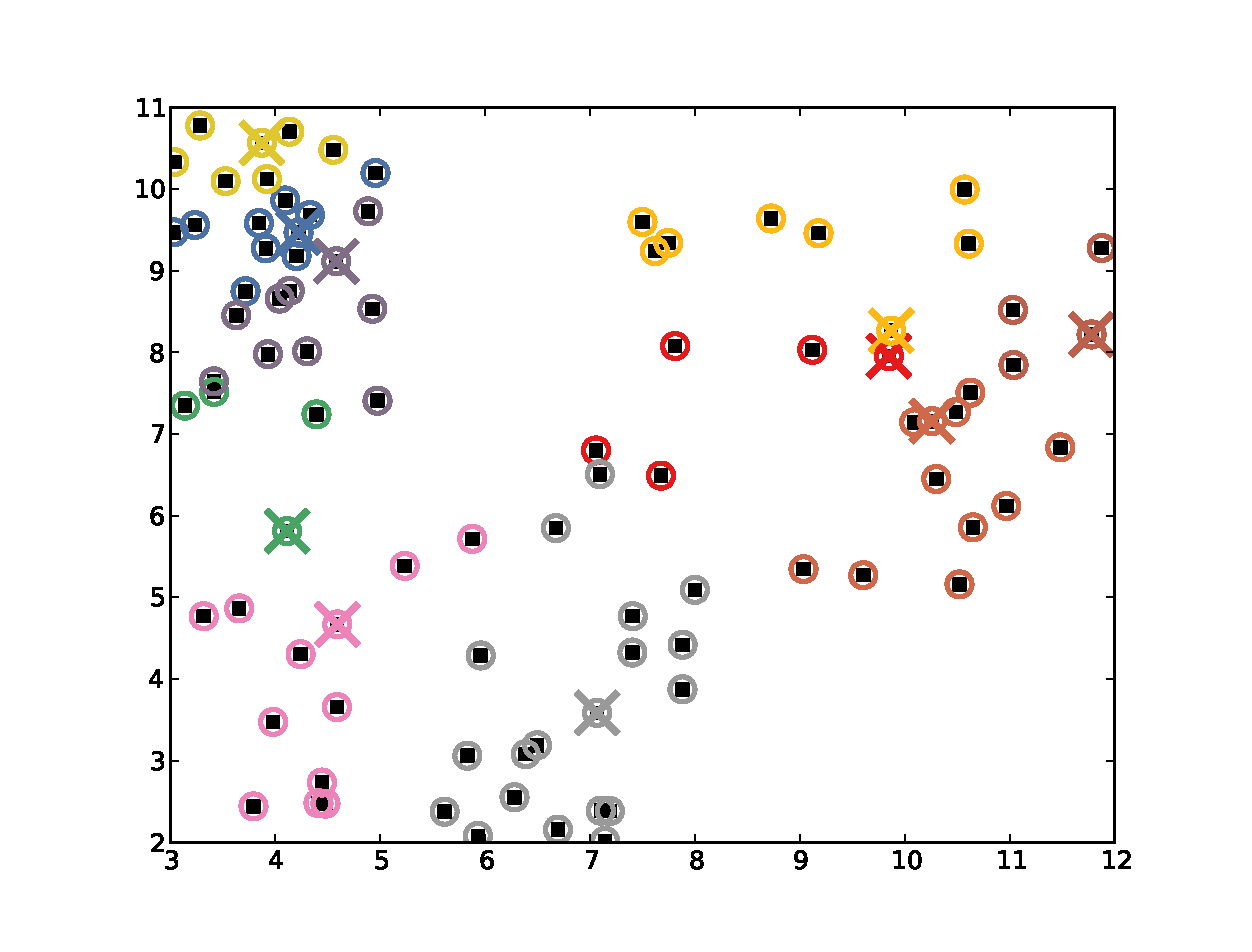
\includegraphics[width=.32\textwidth,height=.3\textheight,keepaspectratio]{figure_8.eps}
    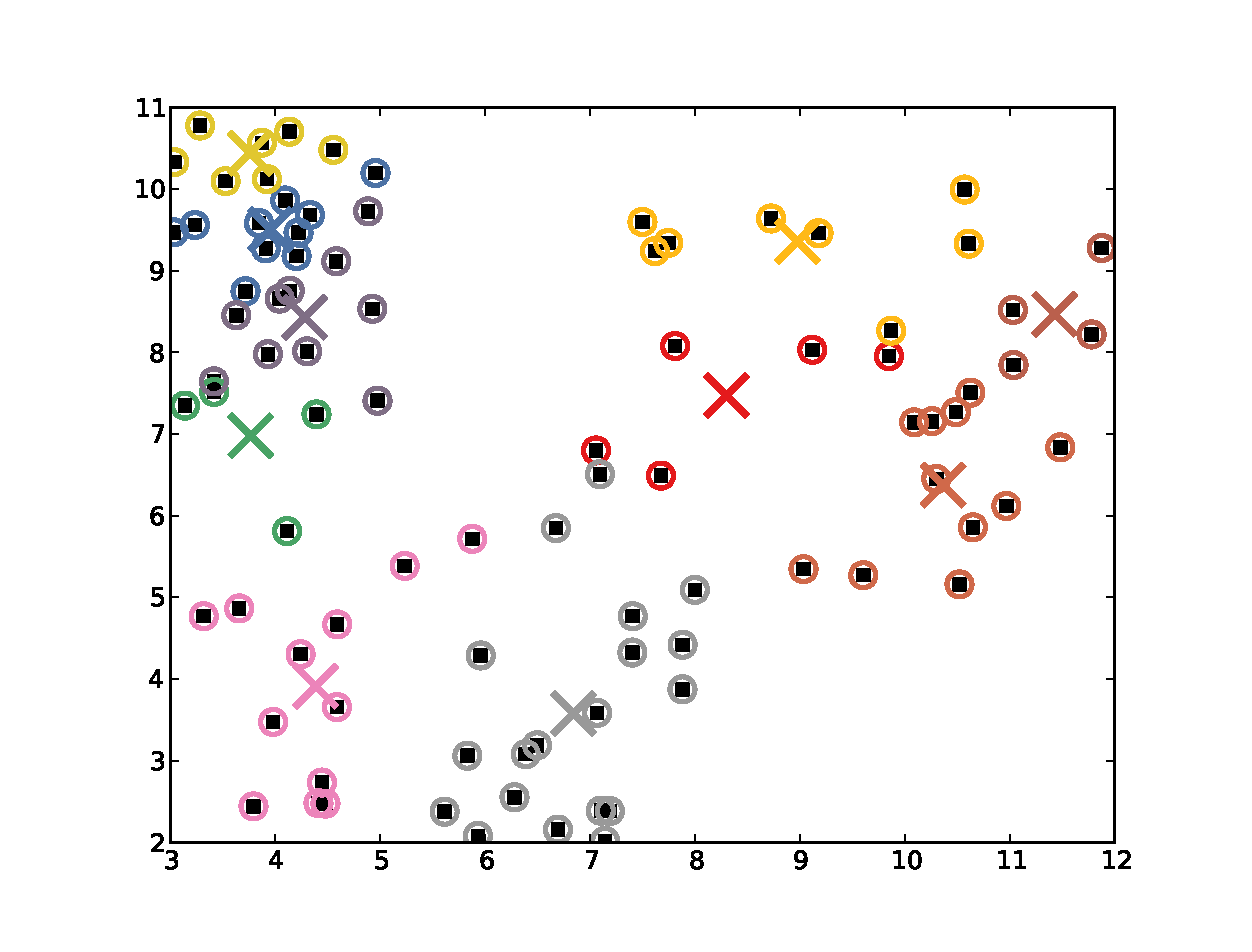
\includegraphics[width=.32\textwidth,height=.3\textheight,keepaspectratio]{figure_9.eps}
    \caption{K=10}
  \end{subfigure}
  \caption{Illustration of the three first steps of the $k$-means algorithm for $k=3,5,10$.}
  \label{fig:kmeanssimple}
\end{figure}

\section{Running your implemented $k$-means}
In this part of the assignment we apply the same algorithm but now use it iteratively. After the new assignment of the center points of the clusters we go to the second step again and we compute new centers. We continue the iterations until a maximum number of iterations is reached. Figure~\ref{fig:kmeansiter} depicts the results of the iterative method for 1, 5, 10 and 20 iterations.  You can see in the figure that the centers are going towards the actual centers of the clusters. However, this is not always the case as the random first step can lead to different results.


\begin{figure}
  \centering
  \begin{subfigure}{.44\textwidth}
    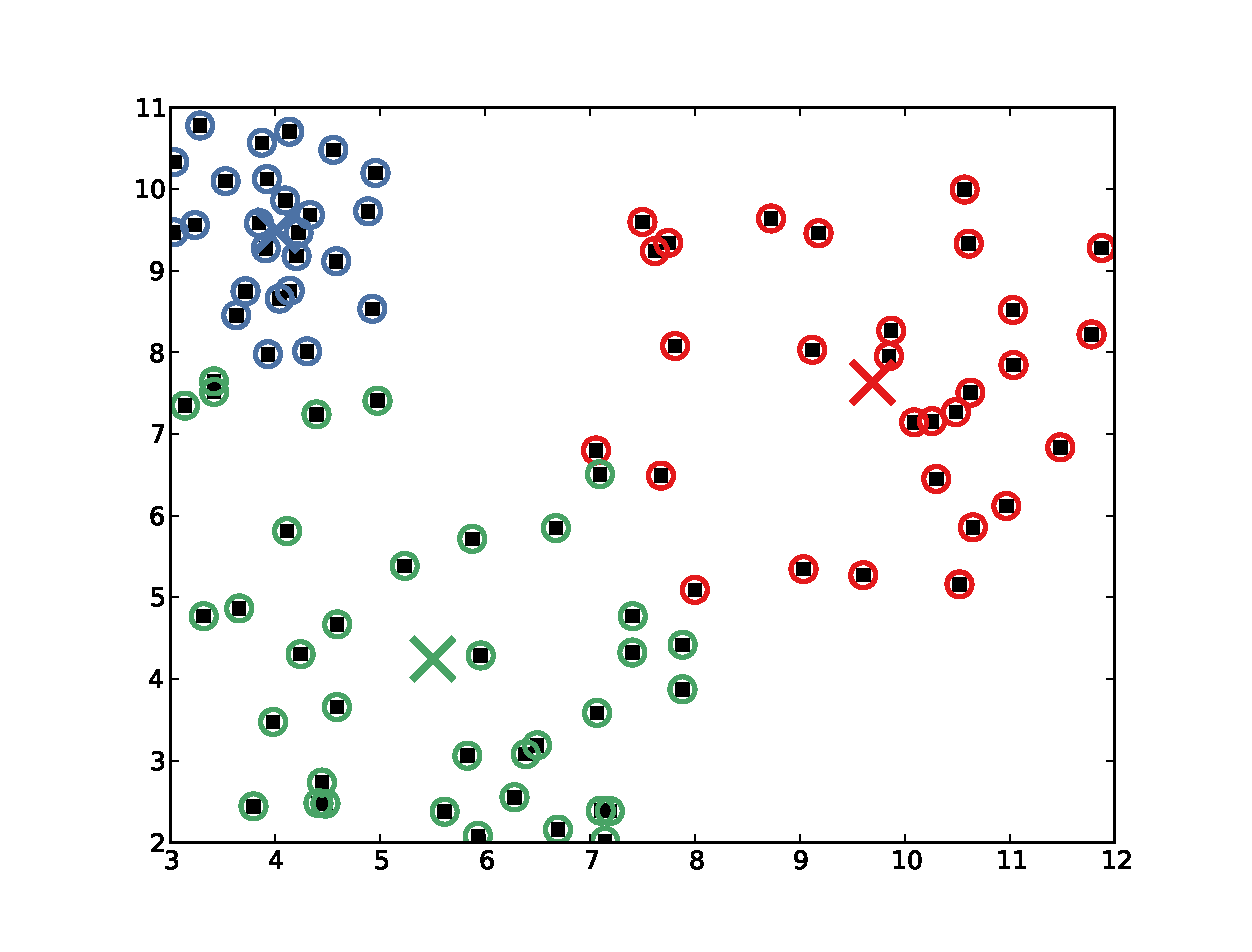
\includegraphics[width=\textwidth,height=.5\textheight,keepaspectratio]{figure_1_1.eps}
    \caption{Iteration level: 1}
  \end{subfigure}
  \hspace*{\fill}
  \begin{subfigure}{.44\textwidth}
    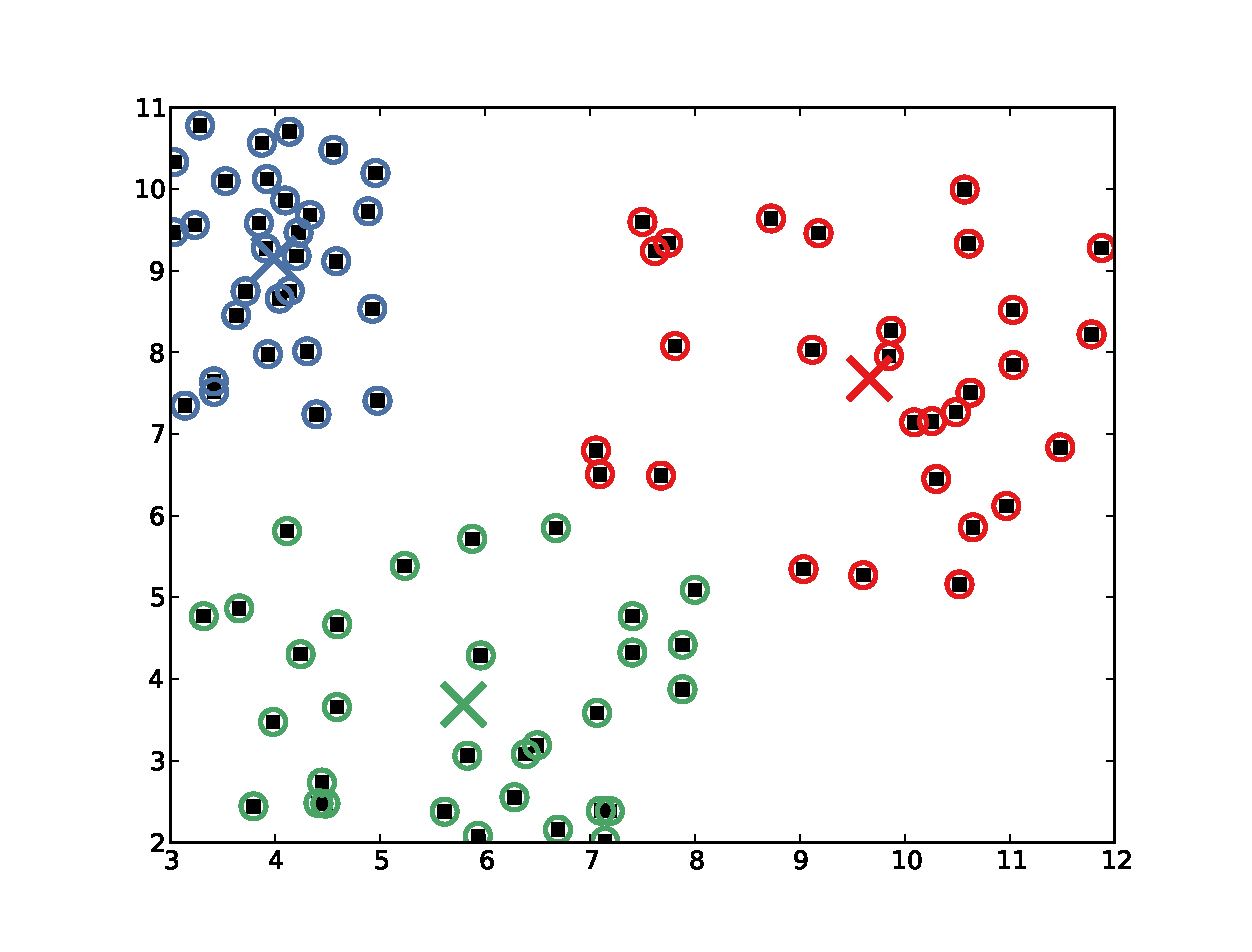
\includegraphics[width=\textwidth,height=.5\textheight,keepaspectratio]{figure_1_2.eps}
    \caption{Iteration level: 5}
  \end{subfigure}

  \begin{subfigure}{.44\textwidth}
    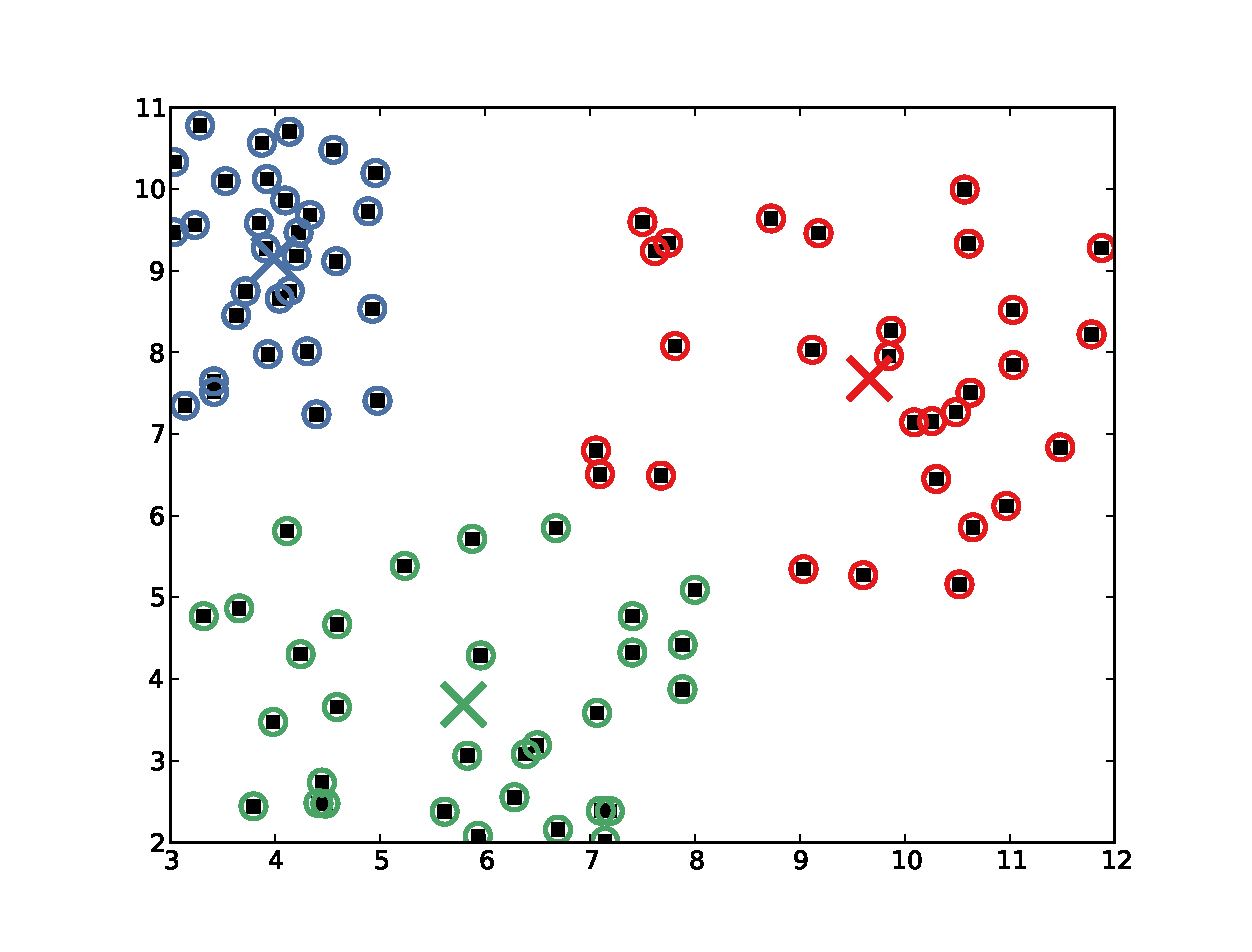
\includegraphics[width=\textwidth,height=.3\textheight,keepaspectratio]{figure_1_3.eps}
    \caption{Iteration level: 10}
  \end{subfigure}
  \hspace*{\fill}
  \begin{subfigure}{.44\textwidth}
    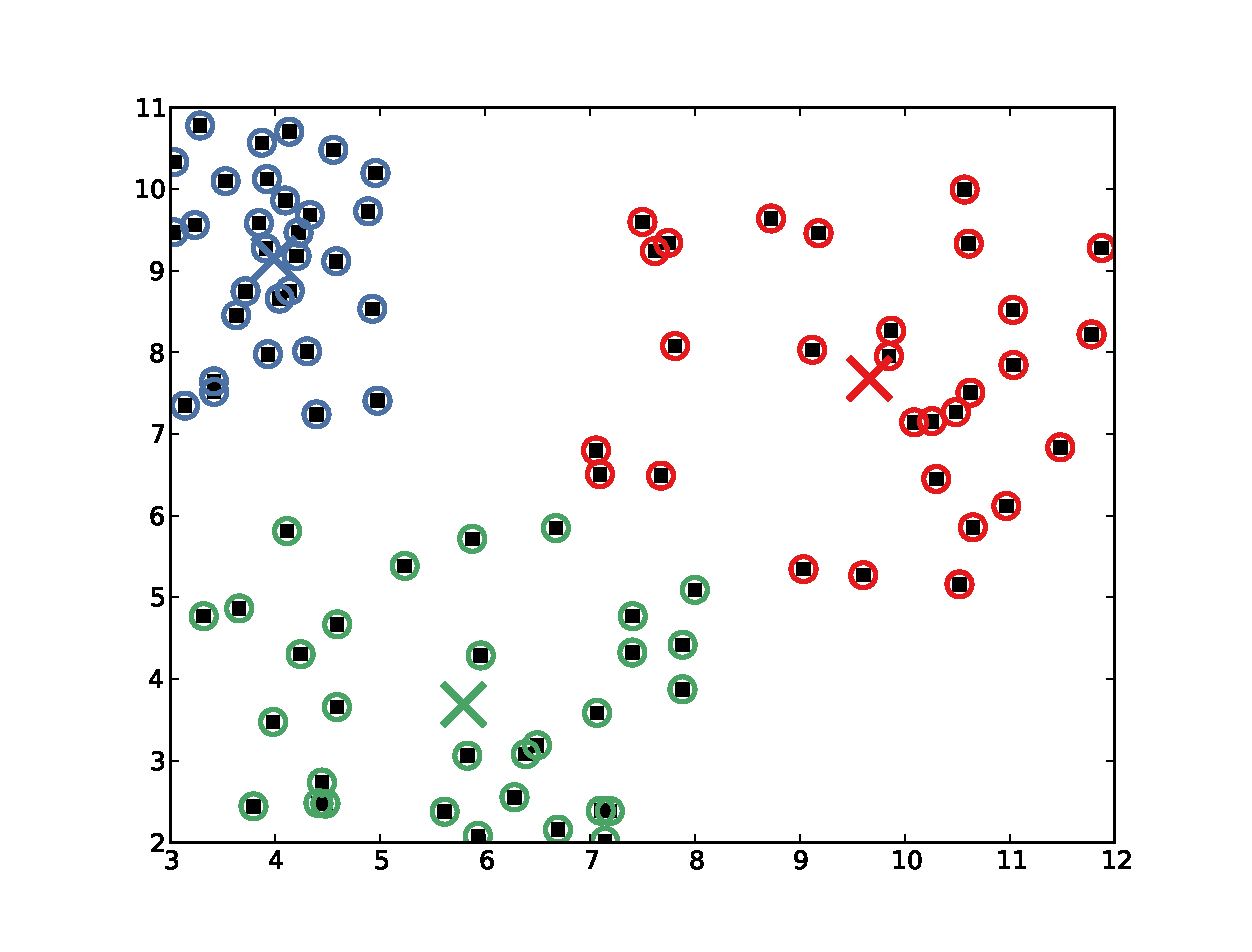
\includegraphics[width=\textwidth,height=.3\textheight,keepaspectratio]{figure_1_4.eps}
    \caption{Iteration level: 20}
  \end{subfigure}

  \caption{Illustration of the iterative $k$-means algorithm for different maximum iterations levels.}%, top left:1, top right:5, bottom left:10, bottom right:20.}
  \label{fig:kmeansiter}
\end{figure}

Apart from reaching a maximum number of iterations, there is another way of stopping the algorithm, and this is done just by computing the distance between the previous centers and the new ones, once the distance has become not large enough to be important we can stop the algorithm. The following part of code is the one that we implemented for this reason.
\begin{verbatim}
new_center_x = center_x/num
new_center_y = center_y/num
new_center_dist = math.sqrt(math.pow(new_center_x - means[i, 0], 2) + 
                  math.pow(new_center_y - means[i, 1], 2))
if new_center_dist > max_change:
   max_change = new_center_dist
   means[i,:] = [new_center_x, new_center_y]
if max_change < 0.001:
    break
\end{verbatim}

\section{Color-based image segmentation}
Now, we apply the same algorithm on actual images. The main idea is the same but now we are dealing with a high dimensional space, so we expect this algorithm to be really slow. Thing that applies especially for large K values. We ran the $k$-means algorithm in the given image for $k = 3, 5, 10, 50, 100$. Figure~\ref{fig:imagekmeans} illustrates the resulting color segments of the image. We can see that for small values for $k$ the image for example $K = 3$, each pixel is assigned a value of one of the three clusters, the resulting image has only three colors and different features in the picture can easily extracted. As the number of clusters increases the clustering is becoming more and more detailed. For $k = 100$ we can hardly see any difference between the clustered and the original image.

\begin{figure}
    \centering
    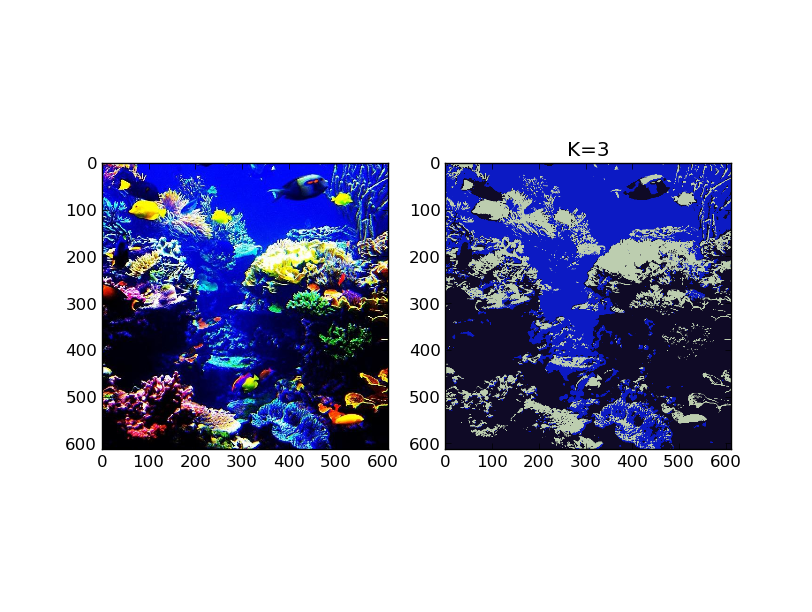
\includegraphics[trim = 1.5cm 3.5cm 1.5cm 3.5cm ,clip=true, width=1.0\textwidth,height=.19\textheight,keepaspectratio]{figure_2_1.png}
    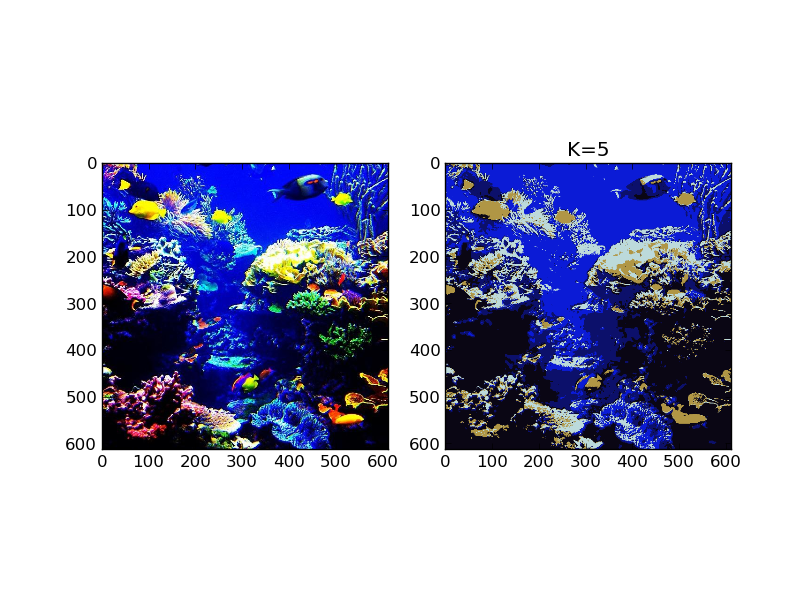
\includegraphics[trim = 1.5cm 3.5cm 1.5cm 3.5cm ,clip=true, width=1.0\textwidth,height=.19\textheight,keepaspectratio]{figure_2_2.png}
    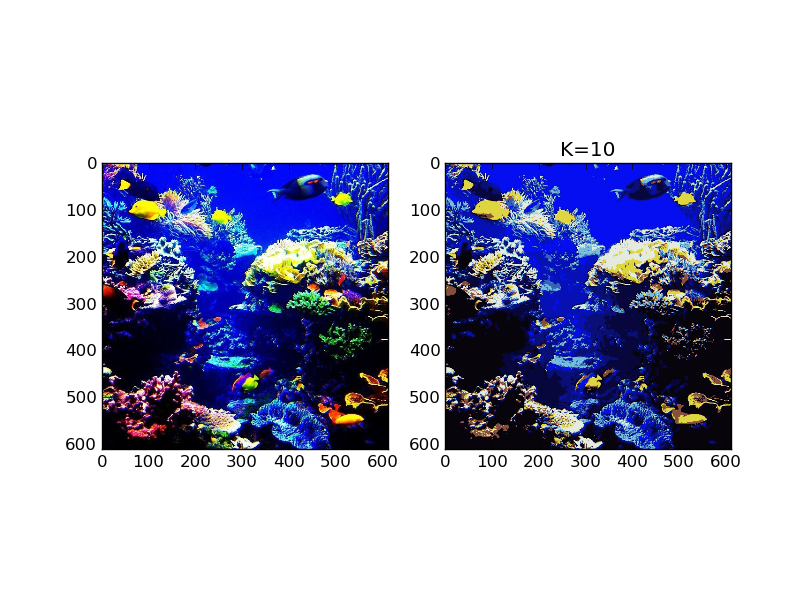
\includegraphics[trim = 1.5cm 3.5cm 1.5cm 3.5cm ,clip=true, width=1.0\textwidth,height=.19\textheight,keepaspectratio]{figure_2_3.png}
    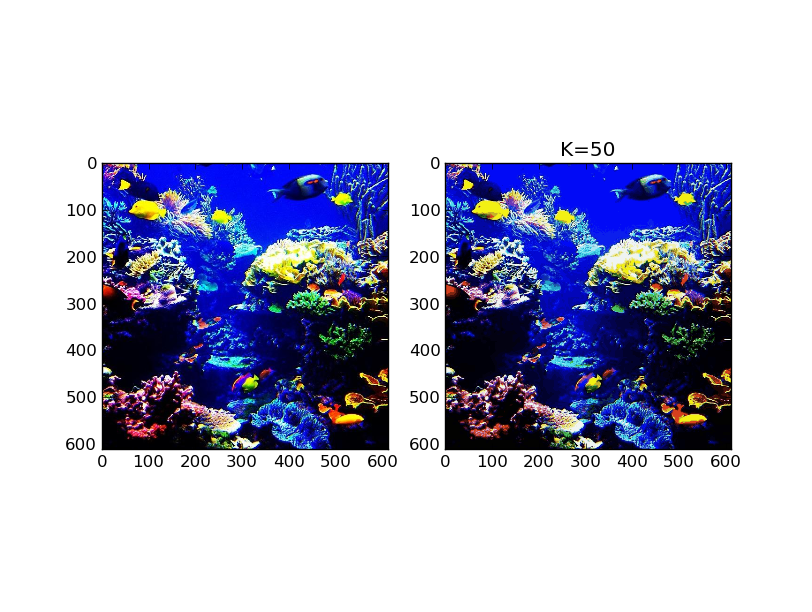
\includegraphics[trim = 1.5cm 3.5cm 1.5cm 3.5cm ,clip=true, width=1.0\textwidth,height=.19\textheight,keepaspectratio]{figure_2_4.png}
    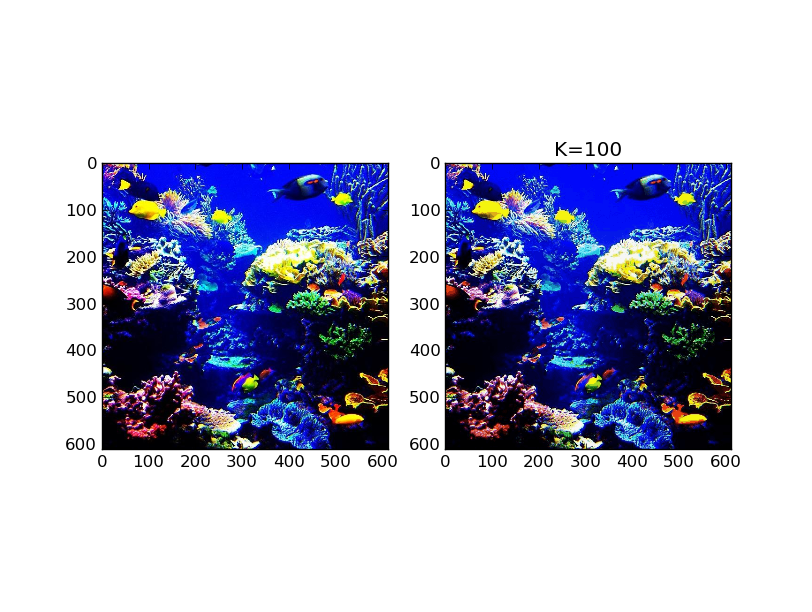
\includegraphics[trim = 1.5cm 3.5cm 1.5cm 3.5cm ,clip=true, width=1.0\textwidth,height=.19\textheight,keepaspectratio]{figure_2_5.png}
  \caption{Illustration of $k$-means algorithm for the above coral image, for $k = 3, 5, 10, 50, 100$.}
  \label{fig:imagekmeans}
\end{figure}

\section{$k$-means, SIFT \& Bag-of-Words: calculating storage for raw SIFT}
Each SIFT vector has 128 elements.  Each element is represented by an integer\footnote{The binary invoked to extract the SIFT vectors returns integers.  However, the \texttt{read\_sift\_from\_file(sift\_path)} function interprets these as Python \texttt{float} objects.  In the standard Python implementation, CPython, a \texttt{float} always consists of 64 bits, which is 8 bytes.  This would result in quadrupling all final answers.}.  Assuming each integer consists of 2 bytes and there is no storage overhead for the vector, 1 SIFT vector needs 256 bytes of storage.  To store all 50,000 vectors that belong to one image, 12,800,000 bytes = $12.8 \cdot 10^6 B = 12.8 \mbox{ MB} \approx 12.21 \mbox{ MiB}$ is needed.  For Facebook's daily addition of new images, one needs $12.8 \cdot 10^6 \cdot 350 \cdot 10^6 \mbox{ B} = 4.48 \cdot 10^{15} \mbox{ B} = 4.48 \mbox{ PB} = 4,480,000,000 \mbox{ MB} = 4272460937.5 \mbox{ MiB} \approx 3.98 \mbox{ PiB}$ of storage.

\section{Visualizing the words on the image, the contents of the words and the Bag-of-Words histograms}
Visual words of five randomly selected images from the dataset have been plotted in Figure~\ref{fig:wordsonimage}.  Note that words tend to be focused on structures that reoccur often, such as lines.  This can be seen in Figure~\ref{sfig:cc85} and~\ref{sfig:as1} at the roof, and in Figure~\ref{sfig:as15} and~\ref{sfig:rc437} at the 3D structures on the wall.

\begin{figure}
  \begin{subfigure}{0.49\textwidth}
    \centering
    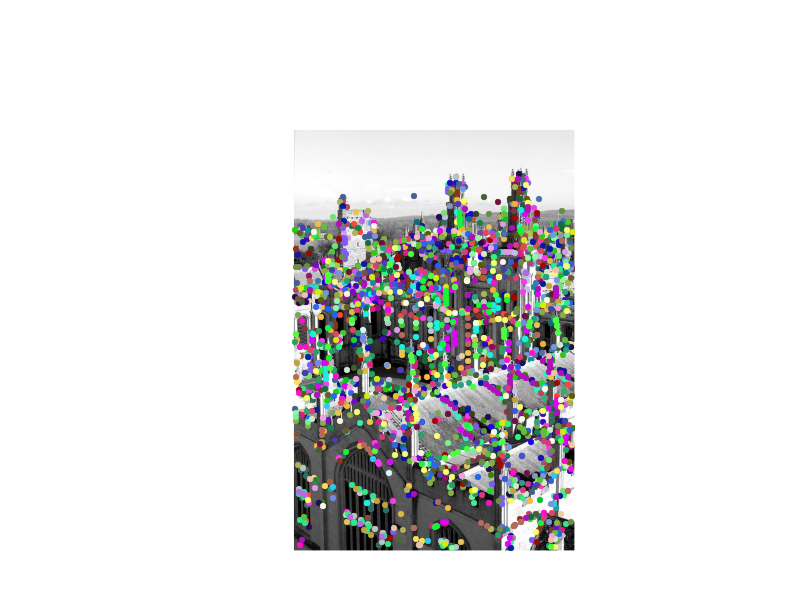
\includegraphics[width=\textwidth,height=.3\textheight,keepaspectratio]{randomimage1}
    \caption{\texttt{christ\_church\_000085.png}}
    \label{sfig:cc85}
  \end{subfigure}
  \begin{subfigure}{0.49\textwidth}
    \centering
    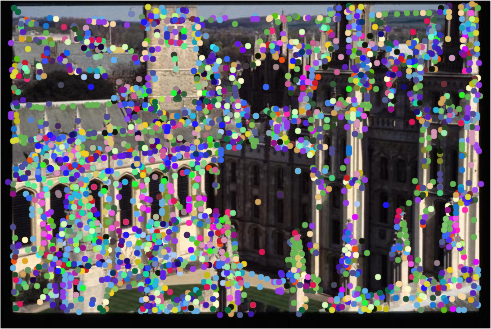
\includegraphics[width=\textwidth,height=.3\textheight,keepaspectratio]{randomimage2}
    \caption{\texttt{all\_souls\_000001png}}
    \label{sfig:as1}
  \end{subfigure}
  \begin{subfigure}{0.49\textwidth}
    \centering
    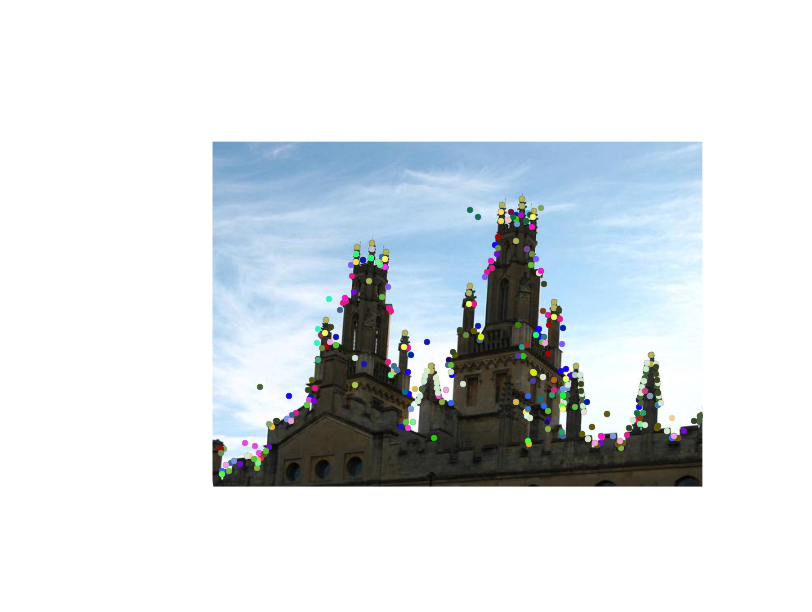
\includegraphics[width=\textwidth,height=.3\textheight,keepaspectratio]{randomimage3}
    \caption{\texttt{all\_souls\_000015png}}
    \label{sfig:as15}
  \end{subfigure}
  \begin{subfigure}{0.49\textwidth}
    \centering
    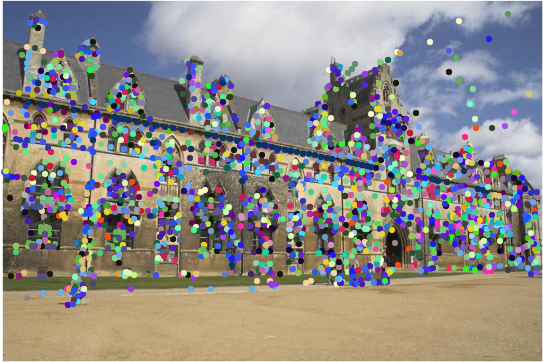
\includegraphics[width=\textwidth,height=.3\textheight,keepaspectratio]{randomimage4}
    \caption{\texttt{christ\_church\_000275png}}
    \label{sfig:cc275}
  \end{subfigure}
  \begin{subfigure}{0.49\textwidth}
    \centering
    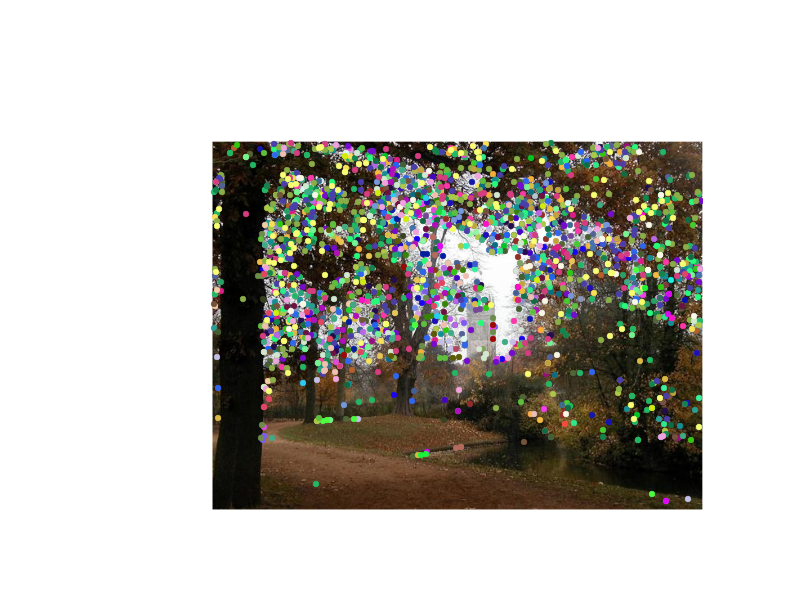
\includegraphics[width=\textwidth,height=.3\textheight,keepaspectratio]{randomimage5}
    \caption{\texttt{radcliffe\_camera\_000437png}}
    \label{sfig:rc437}
  \end{subfigure}
  \begin{subfigure}{0.49\textwidth}
    \centering
    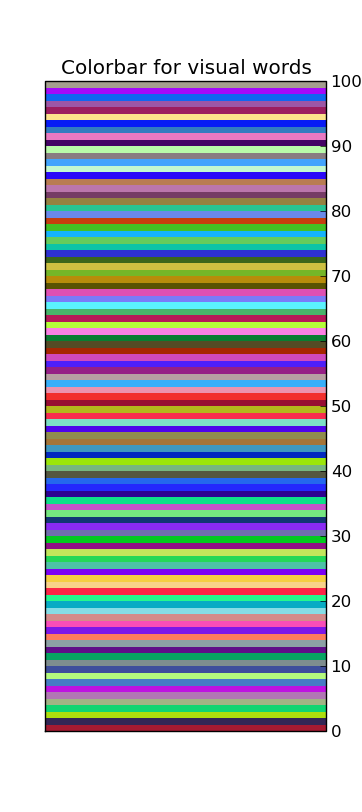
\includegraphics[width=\textwidth,height=.3\textheight,keepaspectratio]{colorbar}
    \caption{Legend.}
    \label{sfig:colorbar}
  \end{subfigure}
  \caption{SIFT vectors that have been assigned to words, plotted on images.  Figure~\ref{sfig:colorbar} functions as a legend for each feature: dots of the same color represent the same SIFT vector.  Its number can be looked up on this bar.}
  \label{fig:wordsonimage}
\end{figure}

The patches of five randomly selected words are shown in Figure~\ref{fig:words}.  The patches do look like each other, when you ignore the differences in hue (but not in intensity), rotation and scale.

\begin{figure}
  \begin{subfigure}{0.49\textwidth}
    \centering
    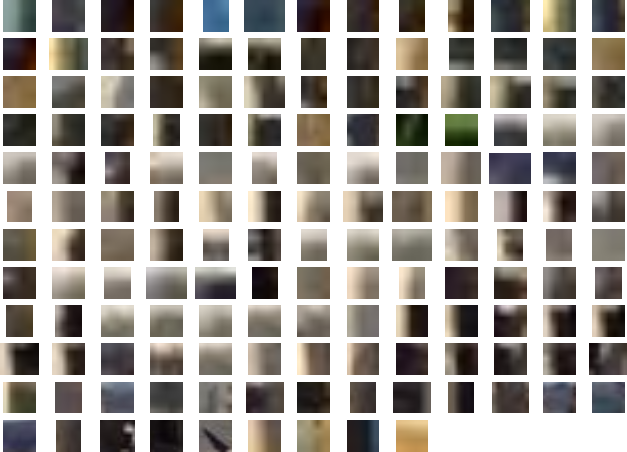
\includegraphics[width=\textwidth,height=.3\textheight,keepaspectratio]{word1}
    \caption{Word 69}
  \end{subfigure}
  \begin{subfigure}{0.49\textwidth}
    \centering
    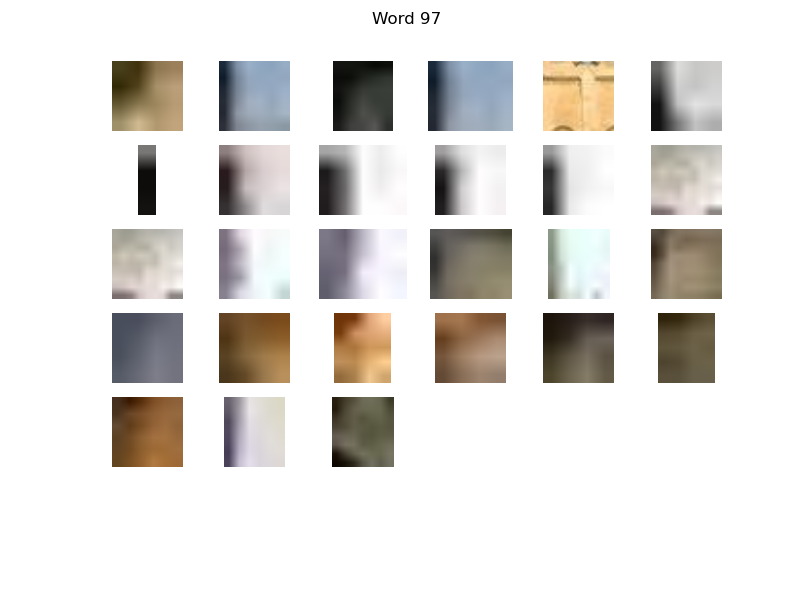
\includegraphics[width=\textwidth,height=.3\textheight,keepaspectratio]{word2}
    \caption{Word 65}
  \end{subfigure}
  \begin{subfigure}{0.49\textwidth}
    \centering
    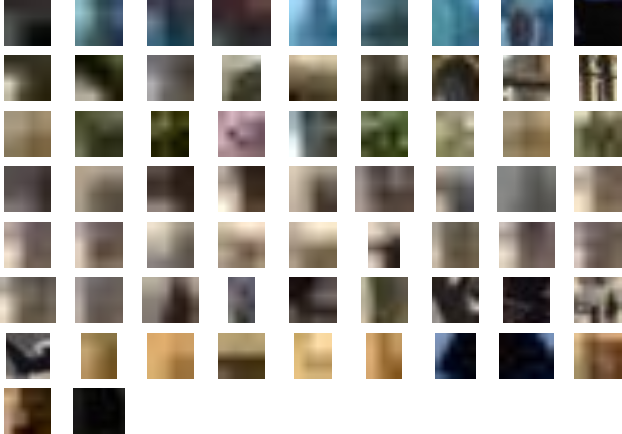
\includegraphics[width=\textwidth,height=.3\textheight,keepaspectratio]{word3}
    \caption{Word 10}
  \end{subfigure}
  \begin{subfigure}{0.49\textwidth}
    \centering
    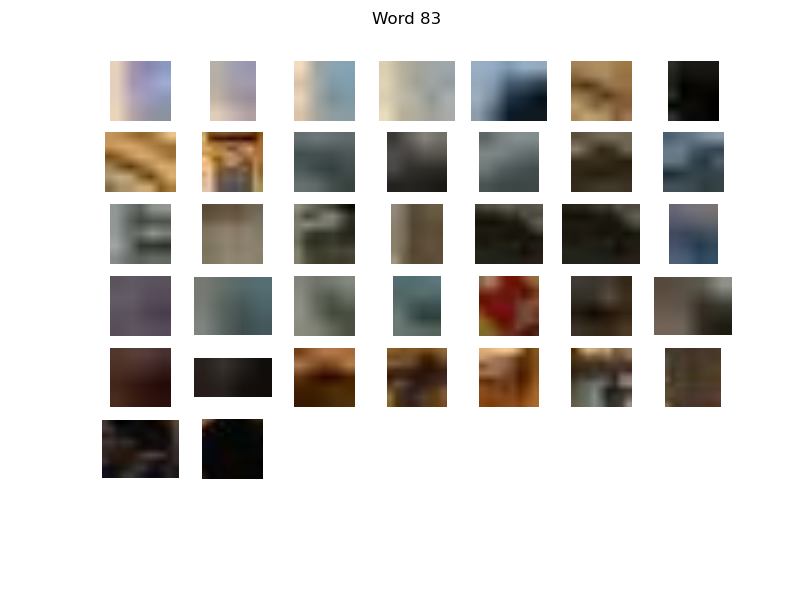
\includegraphics[width=\textwidth,height=.3\textheight,keepaspectratio]{word4}
    \caption{Word 2}
  \end{subfigure}
  \begin{subfigure}{0.49\textwidth}
    \centering
    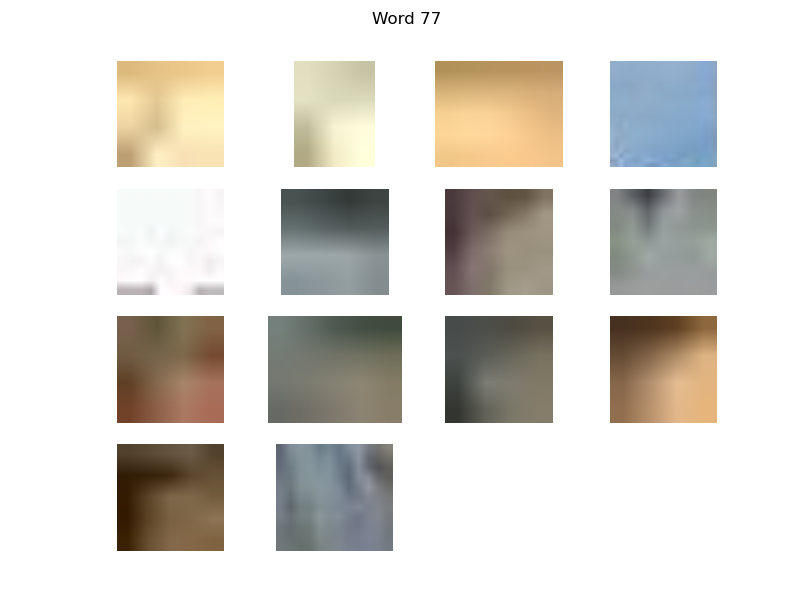
\includegraphics[width=\textwidth,height=.3\textheight,keepaspectratio]{word5}
    \caption{Word 38}
  \end{subfigure}
  \caption{Patches for five randomly selected words, as they occur in the images of Figure~\ref{fig:wordsonimage}.}
  \label{fig:words}
\end{figure}

Finally, the bag-of-words-histogram representation of the images of Figure~\ref{fig:wordsonimage} is presented in Figure~\ref{fig:histograms}.

\begin{figure}
  \begin{subfigure}{0.49\textwidth}
    \centering
    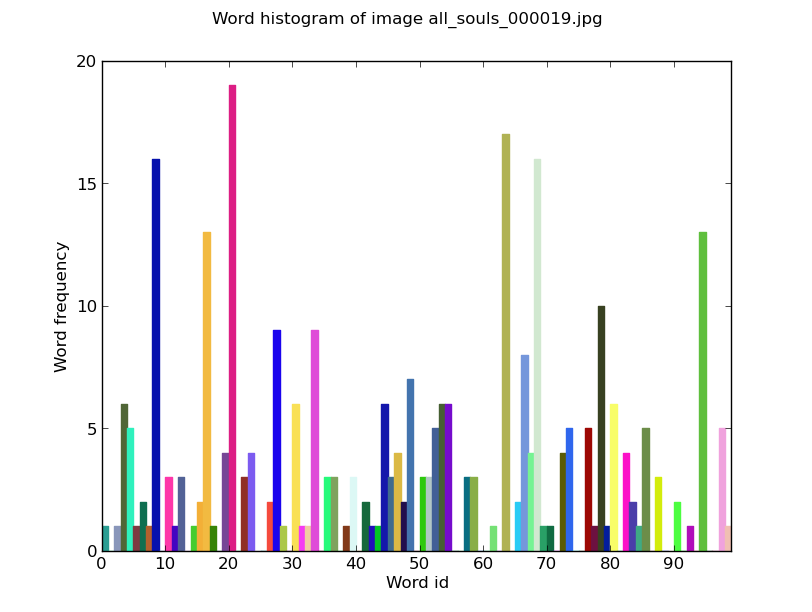
\includegraphics[width=\textwidth,height=.3\textheight,keepaspectratio]{histogram1}
    \caption{\texttt{christ\_church\_000085.png}}
  \end{subfigure}
  \begin{subfigure}{0.49\textwidth}
    \centering
    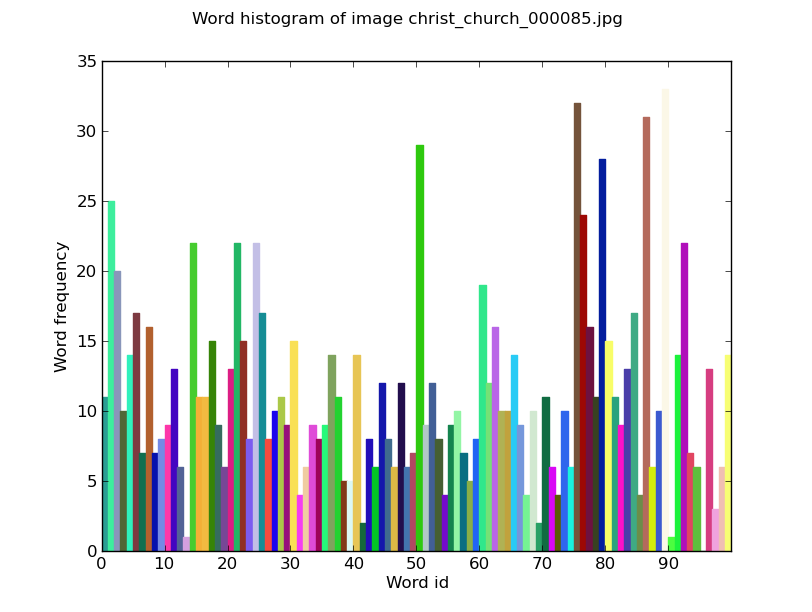
\includegraphics[width=\textwidth,height=.3\textheight,keepaspectratio]{histogram2}
    \caption{\texttt{all\_souls\_000001.png}}
  \end{subfigure}
  \begin{subfigure}{0.49\textwidth}
    \centering
    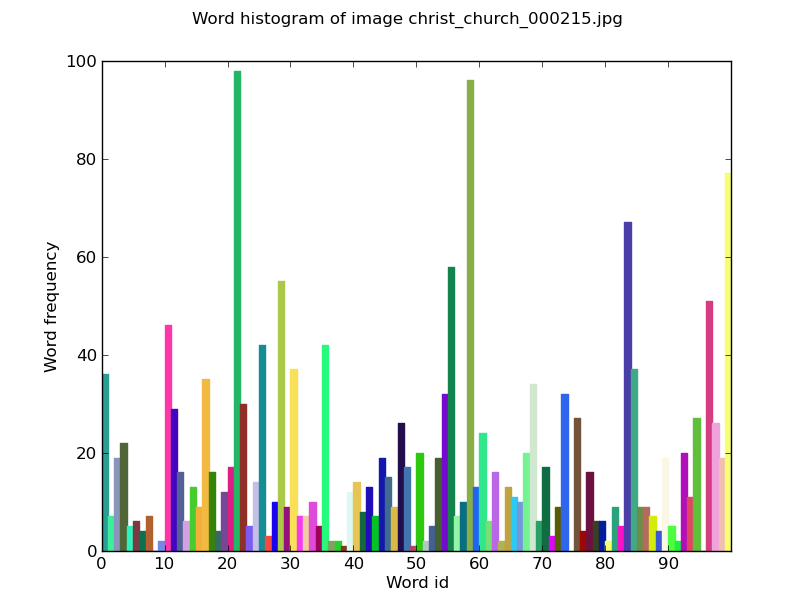
\includegraphics[width=\textwidth,height=.3\textheight,keepaspectratio]{histogram3}
    \caption{\texttt{all\_souls\_000015.png}}
  \end{subfigure}
  \begin{subfigure}{0.49\textwidth}
    \centering
    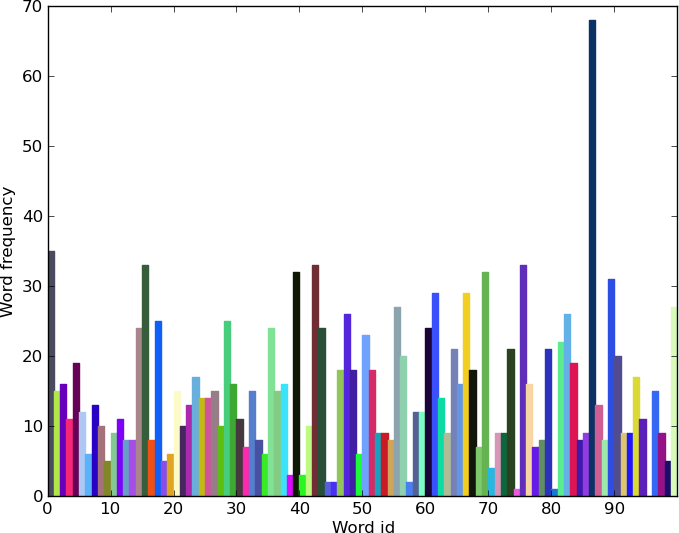
\includegraphics[width=\textwidth,height=.3\textheight,keepaspectratio]{histogram4}
    \caption{\texttt{christ\_church\_000275.png}}
  \end{subfigure}
  \begin{subfigure}{0.49\textwidth}
    \centering
    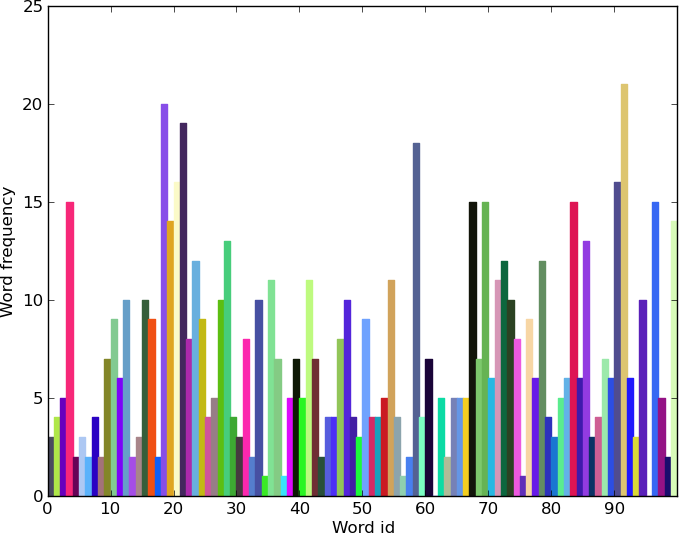
\includegraphics[width=\textwidth,height=.3\textheight,keepaspectratio]{histogram5}
    \caption{\texttt{radcliffe\_camera\_000437.png}}
  \end{subfigure}
  \caption{Frequencies of visual words per image.  Each bar is visualised in the corresponding SIFT vector color.  Figure~\ref{sfig:colorbar} shows these colors.}
  \label{fig:histograms}
\end{figure}

\section{Visualizing Bag-of-Words retrieval}
See Figure~\ref{fig:bow_retrieval} for the ranking.

\begin{figure}
  \begin{subfigure}{0.47\textwidth}
    \centering
    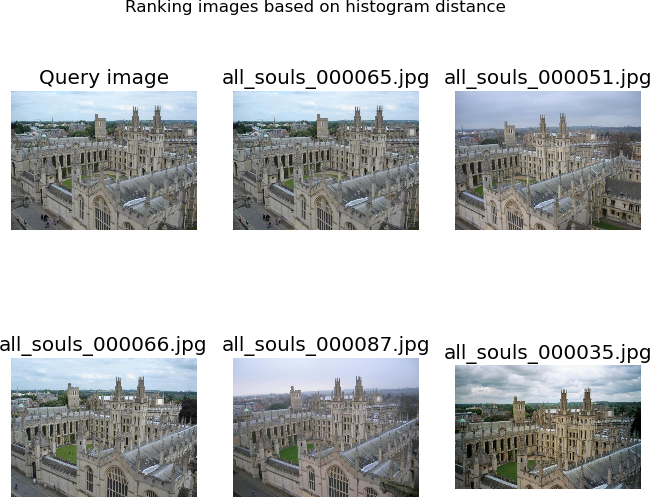
\includegraphics[width=\textwidth]{ranking_h_a}
    \caption{Histogram distance, \texttt{all\_souls\_000065.png}.}
  \end{subfigure}
  \hspace*{\fill}
  \begin{subfigure}{0.47\textwidth}
    \centering
    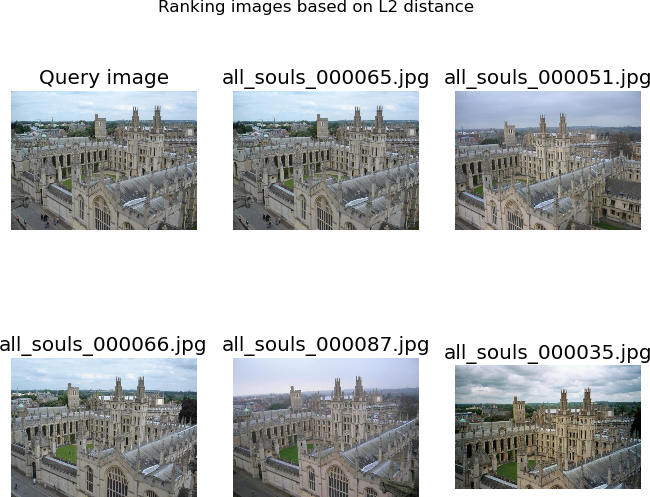
\includegraphics[width=\textwidth]{ranking_l_a}
    \caption{$\ell_2$ distance, \texttt{all\_souls\_000065.png}.}
  \end{subfigure}
  \begin{subfigure}{0.47\textwidth}
    \centering
    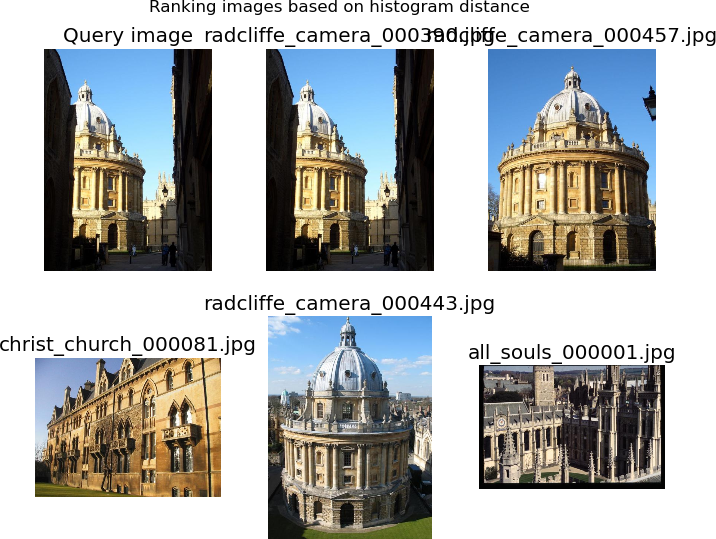
\includegraphics[width=\textwidth]{ranking_h_r}
    \caption{Histogram distance, \texttt{radcliffe\_camera\_000390.png}.}
  \end{subfigure}
  \hspace*{\fill}
  \begin{subfigure}{0.47\textwidth}
    \centering
    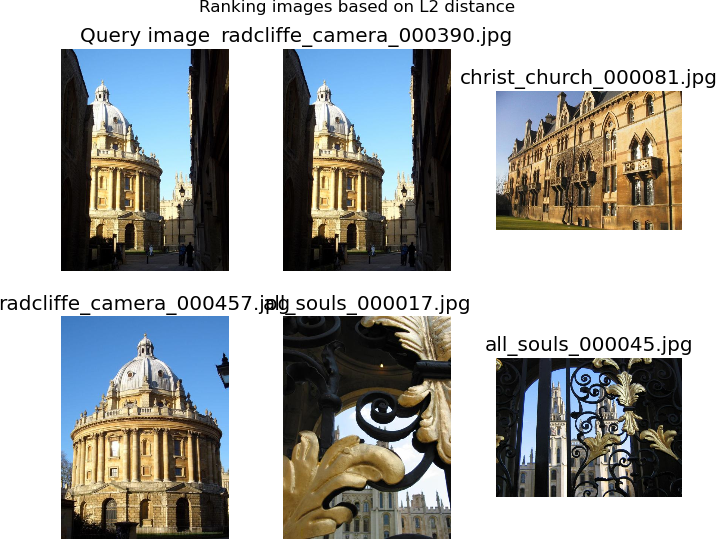
\includegraphics[width=\textwidth]{ranking_l_r}
    \caption{$\ell_2$ distance, \texttt{radcliffe\_camera\_000390.png}.}
  \end{subfigure}
  \begin{subfigure}{0.47\textwidth}
    \centering
    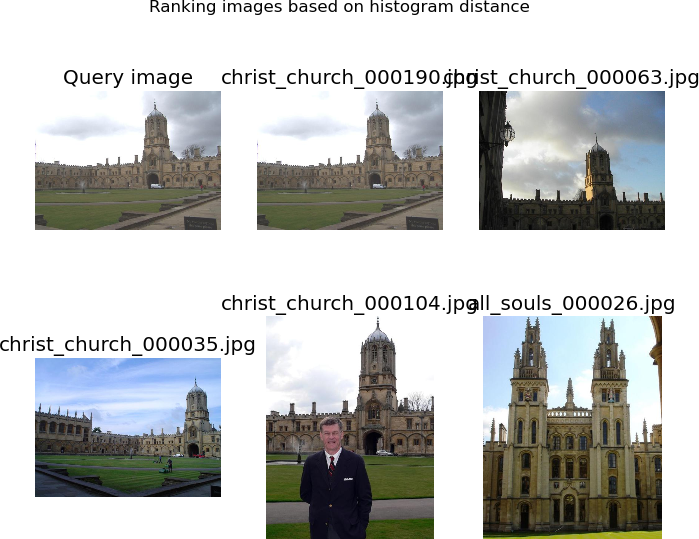
\includegraphics[width=\textwidth]{ranking_h_c}
    \caption{Histogram distance, \texttt{christ\_church\_000190.png}.}
  \end{subfigure}
  \hspace*{\fill}
  \begin{subfigure}{0.47\textwidth}
    \centering
    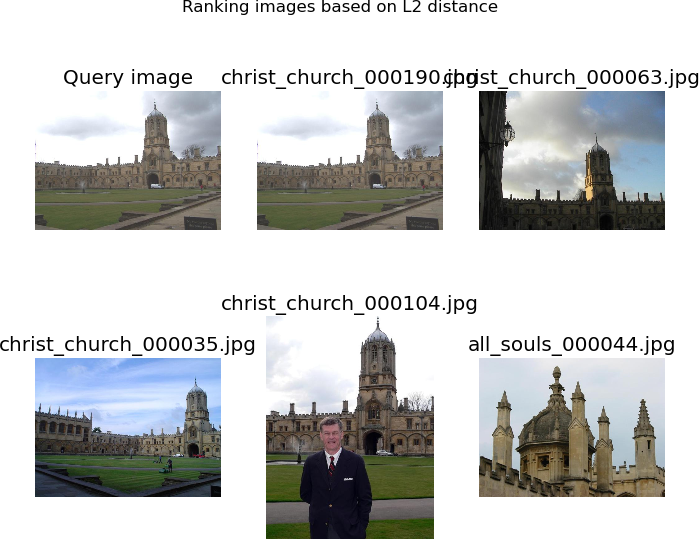
\includegraphics[width=\textwidth]{ranking_l_c}
    \caption{$\ell_2$ distance, \texttt{christ\_church\_000190.png}.}
  \end{subfigure}
  \caption{Ranking of retrieved images based on different distance measures between histograms of bags of words.}
  \label{fig:bow_retrieval}
\end{figure}

\section{Evaluating Bag-of-Words histograms}
Precision scores of the bag of words retrieval system can be found in Figure~\ref{fig:precision}.  Precision scores of the color histogram retrieval system for the same images can be found in table~\ref{tab:color_precision}.  The precision of the bag of words retrieval system seems to have an optimum for the codebook size.  Smaller codebooks such as 5 and 10 seem to perform at least equally well in most cases as larger codebooks such as 500 and 1000.  No strong conclusions can be made based on the current observations, as only a small number of queries have been examined, but this seems to tend towards overfitting; the data representation becomes too specific.

From the average precision scores, we might be able to conclude that the histogram distance performs better than the $\ell_2$ distance, especially when few images need to be retrieved.

We might also conclude that there are very few images like \texttt{christ\_church\_000190}, as neither measure returns high precision.  

To propose a method to improve the accuracy of the system, we should investigate the current accuracy as well, which has not been done. A method to improve the precision might be to use a different feature descriptor than SIFT.  One might want to look at histograms of oriented gradients, SURF or AGAST.

Comparing the bag of words retrieval system with the color histogram retrieval system, we can observe that only in a few cases the color histogram system outperforms the bag of words system.  In general, the bag of words system outperforms the color histogram system.  This is not that strange; the bag of words system is based on a more advanced feature descriptor method than color histograms.

\begin{figure}
  \begin{subfigure}{0.47\textwidth}
    \centering
    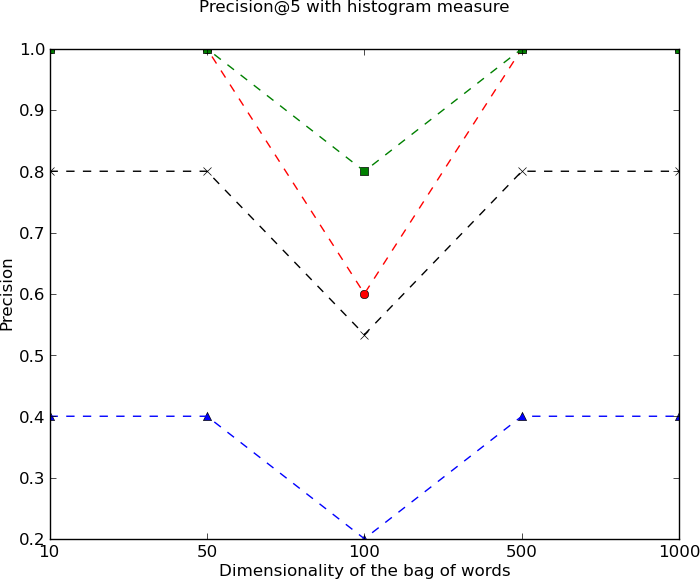
\includegraphics[width=\textwidth]{p5h}
    \caption{Precision@5, histogram distance.}
  \end{subfigure}
  \hspace*{\fill}
  \begin{subfigure}{0.47\textwidth}
    \centering
    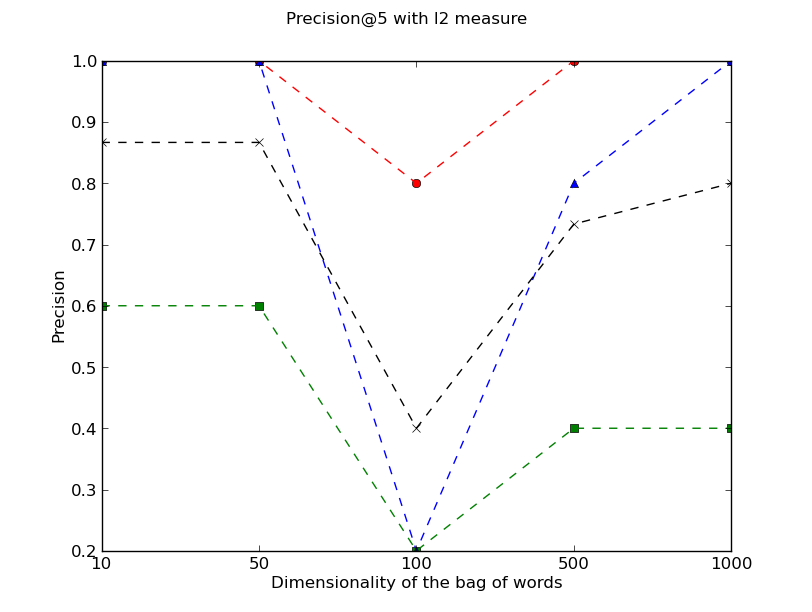
\includegraphics[width=\textwidth]{p5l}
    \caption{Precision@5, $\ell_2$ distance.}
  \end{subfigure}
  \begin{subfigure}{0.47\textwidth}
    \centering
    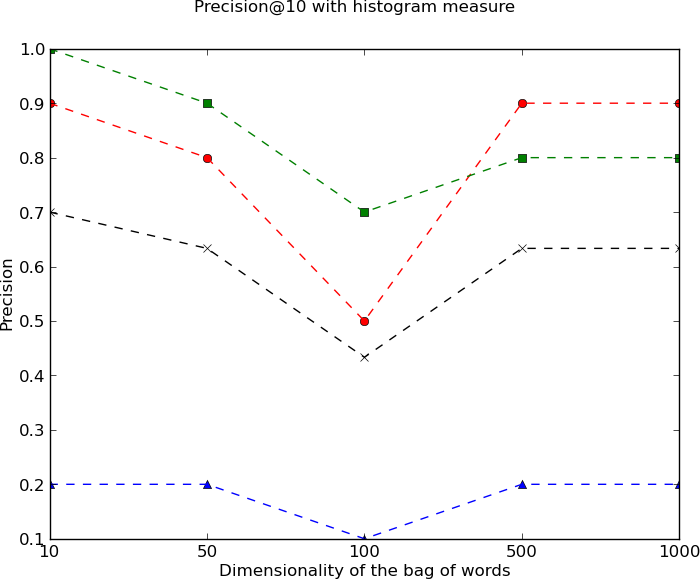
\includegraphics[width=\textwidth]{p10h}
    \caption{Precision@10, histogram distance.}
  \end{subfigure}
  \hspace*{\fill}
  \begin{subfigure}{0.47\textwidth}
    \centering
    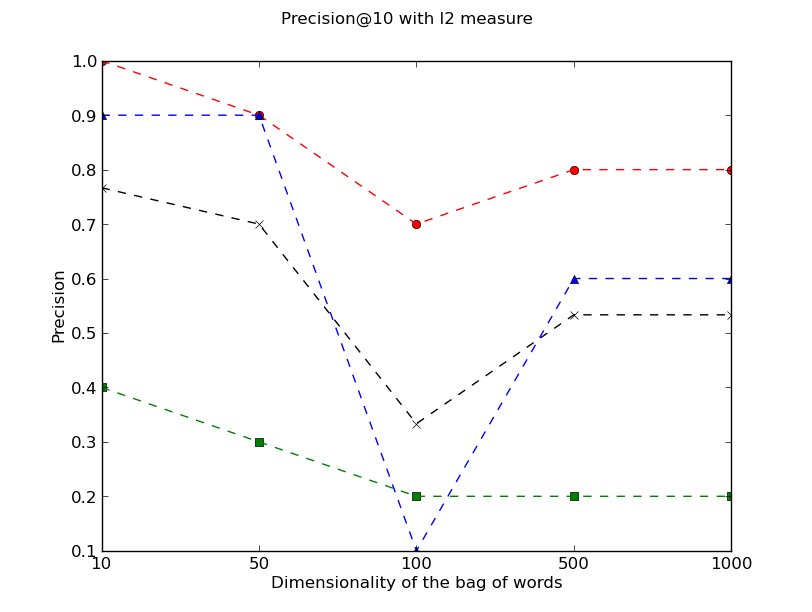
\includegraphics[width=\textwidth]{p10l}
    \caption{Precision@10, $\ell_2$ distance.}
  \end{subfigure}
  \caption{Precision@5 and precision@10 with histogram and $\ell_2$ distance measures for the bag of words retrieval system.  Results are shown for three different images, and their average scores.  Red circles represent scores for \texttt{all\_souls\_000065}, green squares display values for \texttt{radcliffe\_camera\_000390}, blue triangles those of \texttt{christ\_church\_000190}, and black crosses stand for the average values.}
  \label{fig:precision}
\end{figure}

\begin{table}
  \begin{subtable}{0.47\textwidth}
    \begin{tabular}{l|l}
      \texttt{all\_souls\_000065} & $0.8$ \\
      \texttt{radcliffe\_camera\_000390} & $0.4$ \\
      \texttt{christ\_church\_000190} & $0.2$ \\
      \hline
      Average                     & $0.47$ \\
    \end{tabular}
    \caption{Precision@5, histogram distance.}
    \label{tab:color_p5h}
  \end{subtable}
  \hspace*{\fill}
  \begin{subtable}{0.47\textwidth}
    \begin{tabular}{l|l}
      \texttt{all\_souls\_000065} & $0.6$ \\
      \texttt{radcliffe\_camera\_000390} & $0.0$ \\
      \texttt{christ\_church\_000190} & $0.0$ \\
      \hline
      Average                     & $0.2$ \\
    \end{tabular}
    \caption{Precision@5, $\ell_2$ distance.}
    \label{tab:color_p5l}
  \end{subtable}
  \begin{subtable}{0.47\textwidth}
    \begin{tabular}{l|l}
      \texttt{all\_souls\_000065} & $0.5$ \\
      \texttt{radcliffe\_camera\_000390} & $0.3$ \\
      \texttt{christ\_church\_000190} & $0.1$ \\
      \hline
      Average                     & $0.3$ \\
    \end{tabular}
    \caption{Precision@10, histogram distance.}
    \label{tab:color_p10h}
  \end{subtable}
  \hspace*{\fill}
  \begin{subtable}{0.47\textwidth}
    \begin{tabular}{l|l}
      \texttt{all\_souls\_000065} & $0.4$ \\
      \texttt{radcliffe\_camera\_000390} & $0.1$ \\
      \texttt{christ\_church\_000190} & $0.2$ \\
      \hline
      Average                     & $0.23$ \\
    \end{tabular}
    \caption{Precision@10, $\ell_2$ distance.}
    \label{tab:color_p10l}
  \end{subtable}
  \caption{Precision@5 and precision@10 with histogram and $\ell_2$ distance measures for the color histogram retrieval system.  Results are shown for three different images, and their average scores.}
  \label{tab:color_precision}
\end{table}

\bibliographystyle{plain}
\bibliography{thereference}
\end{document}
